\section{Why do we study calculus?} \label{S:0.1}

\begin{goals}
\item What is the behavior of a function arbitrarily close to, but not necessarily at, a specific point?
\item Given a specific input in the domain of a function, what is the instantaneous rate of change of the function at that point?
\item Given a function that represents the rate of change of some quantity over a specific time interval, how much of that quantity has accumulated over that time interval?
\item How are instantaneous rate of change and accumulation related?
\end{goals}

%--------------------------------------
% SUBSECTION INTRODUCTION
%--------------------------------------
\subsection*{Introduction}

Calculus is all about answering these Motivating Questions for all functions in general, but let's first consider piece-wise linear functions so that we may illustrate the ideas of questions two and three.    

Let's start with a car that's driving on a long, flat, straight road.  Instead of having a speedometer and odometer, the car is equipped with a {\em velocitometer} and {\em positometer}.  A velocitometer measures velocity, which is positive when the car moves forward, negative when the car moves backward, and zero when the car is at rest.  A positometer measures position away from some starting point--typically the origin, which may be positive, negative, or zero.
\begin{marginfigure}[-2in] % MARGIN FIGURE
\begin{center}
{\scalebox{.5}{\input{figs/0/velocitometer.pdf_t}}}
\caption{A velocitometer with positometer.}
\label{fig:velocitometer}
\end{center}
\end{marginfigure}

We'll denote the velocity with $v$, which will have units measured in miles per hour, and we'll denote the position with $s$, which will have units measured in miles.

Suppose the position of the car increases linearly such that at time $t=2$, the position is $110$ miles, and at time $t=4$, the position is $220$ miles.  Notice that since this function is a straight line, or linear, we can compute its slope, which is the rate of change of a linear function.  The slope is
\begin{eqnarray*}
v	& = & \frac{\mbox{change in position}}{\mbox{change in time}} = \frac{220 \mbox{ miles} - 110 \mbox{ miles}}{4 \mbox{ hours} - 2 \mbox{ hours}} \\
	& = & \frac{110 \mbox{ miles}}{2 \mbox{ hours}} = 55 \mbox{ miles per hour.}
\end{eqnarray*}
As you can see in the equation above, we used $v$ to denote the slope instead of the usual $m$.  That's because velocity is defined exactly to be the ratio of the change in position to the change of time.

\begin{marginfigure}[-2.5in] % MARGIN FIGURE
\includegraphics[width=\marginparwidth]{figs/0/linear_position_function.pdf}
\caption{A linear position function.}
\label{fig:0-linear_position_function}
\end{marginfigure}

Also notice that with linear functions, the slope is constant, meaning the slope is the same at every point and over every interval.  So if we wish to know the average or instantaneous rate of change of a linear function, we simply need to calculate the slope of the line!

\begin{marginfigure}[1in] % MARGIN FIGURE
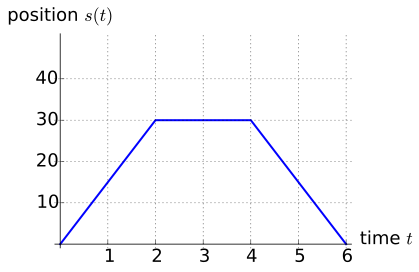
\includegraphics[width=\marginparwidth]{figs/0/piecewise_linear_position_function.pdf}
\caption{A piece-wise linear position function.}
\label{fig:0-piecewise_linear_position_function}
\end{marginfigure}

\begin{example} % EXAMPLE
Use Figure \ref{fig:0-piecewise_linear_position_function} to determine the instantaneous rate of change, or velocity, of the car at $t = 1$, $t = 3$, and $t = 5$. 

\solution When $t = 1$, the position of the car is determined by the line segment passing through the points $(0,0)$ and $(2,3)$.  The slope of that segment is then
\[ \mbox{slope} = \frac{30 - 0}{2 - 0} = \frac{30}{2} = 15, \]
and so the instantaneous rate of change of the car is 15 miles per hour at $t = 1$.

When $t = 3$, the position of the car is determined by the line segment passing through the points $(2,30)$ and $(4,30)$.  The slope of that segment is
\[ \mbox{slope} = \frac{30 - 30}{4 - 2} = 0, \]
and so the instantaneous rate of change of the car is 0 miles per hour at $t = 3$.

Finally, when $t = 5$, the position of the car is determined by the line segment passing through the points $(4,30)$ and $(6,0)$.  The slope of that segment is then
\[ \mbox{slope} = \frac{30 - 0}{4 - 6} = \frac{30}{-2} = -15, \]
and so the instantaneous rate of change of the car is $-15$ miles per hour at $t = 5$.
\end{example}

Now suppose the velocity of the car is constant at $v = 55$ miles per hour starting at time $t=0$. If we wanted to find the position of the car after $t=3$ hours, then we would simply use the equation
\begin{eqnarray*}
\mbox{position}	& = & \mbox{rate} \times \mbox{time} \\
& = & 55 \mbox{ miles per hour} \times 3 \mbox{ hours} \\
& = & 165 \mbox{ miles.} 
\end{eqnarray*}

\begin{marginfigure} % MARGIN FIGURE
\margingraphics{figs/0/constant_velocity_function.pdf}
\caption{The constant velocity function.}
\label{fig:0-constant_velocity_function}
\end{marginfigure}

\begin{marginfigure} % MARGIN FIGURE
\captionsetup[subfigure]{labelformat=empty}
\subfloat{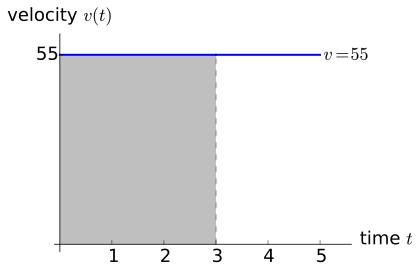
\includegraphics[width=\marginparwidth]{figs/0/position_t3.pdf}}

\subfloat{\includegraphics[width=\marginparwidth]{figs/0/position_t5.pdf}}
\caption{Position at $t=3$ and $t=5$ represented by the area of a rectangle.}
\label{fig:0-position_t5}
\end{marginfigure}

\begin{marginfigure}[.5in] % MARGIN FIGURE
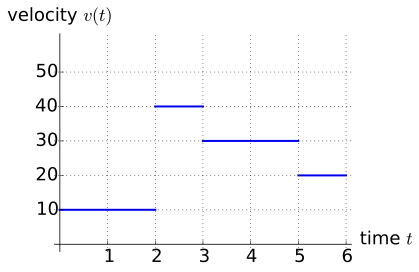
\includegraphics[width=\marginparwidth]{figs/0/piecewise_constant_velocity.pdf}
\caption{A piece-wise constant velocity function.}
\label{fig:0-piecewise_constant_velocity}
\end{marginfigure}

After $5$ hours, the postion would be
\begin{eqnarray*}
\mbox{position}	& = & \mbox{rate} \times \mbox{time} \\
& = & 55 \mbox{ miles per hour} \times 5 \mbox{ hours} \\
& = & 275 \mbox{ miles.} 
\end{eqnarray*}

Geometrically, we can represent the position of the car after 3 hours by the area of the rectangle created by the constant function $v(t) = 55$, the $t$-axis, and the vertical lines $t = 0$ and $t = 3$.  Similarly, we can represent the position after 5 hours geometrically as the area of the region bounded by the $t$-axis and $v(t) = 55$ from $t = 0$ to $t = 5$.  Notice that  region is also a rectangle with height equal to $55$ and width equal to $5 - 0 = 5$.

So in general, if we have a piece-wise constant function--a function consisting of segments of horizontal lines--that represents the velocity of the car (or any other object!), then we can find the position of the car at time $t$ by summing the areas of the rectangles underneath the piece-wise constant function from time $0$ to time $t$.

\begin{example} % EXAMPLE
Use Figure \ref{fig:0-piecewise_constant_velocity} to determine the position of the car at time $t=6$.

\solution In the figure, there are four horizontal line segments that comprise the piece-wise constant function.  So there will be four rectangles whose areas we must calculate, and then we will sum those areas to determine the position of the car at $t=6$.

From $t = 0$ to $t = 2$, the rectangle has height $10$ and width $2$; therefore, its area is $10 \times 2 = 20$.

From $t = 2$ to $t = 3$, the rectangle has height $40$ and width $1$; therefore, its area is $40 \times 1 = 40$.

From $t = 3$ to $t = 5$, the rectangle has height $30$ and width $2$; therefore, its area is $30 \times 2 = 60$.

And from $t = 5$ to $t = 6$, the rectangle has height $20$ and width $1$; therefore, its area is $20 \times 1 = 20$.

So the position of the car at $t = 6$ is $20 + 40 + 60 + 20 = 140$ miles.
\end{example}

What if the velocity function is a piece-wise linear function instead of a piece-wise constant function as seen in Figure~\ref{fig:0-piecewise_linear_velocity}?  Nothing changes with respect to {\em how} we find the position--we still must find the area underneath the function, but the region(s) may not be rectangular.  They may be triangles, trapezoids, or rectangles, which means we may need to remember the area formulas for those polygons.  But it is certainly possible to calculate the position from a piece-wise linear velocity function using only algebra.

\begin{marginfigure} % MARGIN FIGURE
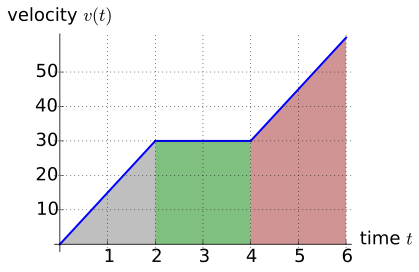
\includegraphics[width=\marginparwidth]{figs/0/piecewise_linear_velocity.pdf}
\caption{A piece-wise linear velocity function.}
\label{fig:0-piecewise_linear_velocity}
\end{marginfigure}

\concept{Slope and Area}{ % CONCEPT
The slope of the position graph $s$ at some point gives the velocity $v$ at that point. The area of the region underneath the velocity graph $v$ from time $0$ to time $t$ gives the position $s$ at time $t$.
}% end concept

So what if we wish to find the instantaneous rate of change, or slope, of a function that is not piece-wise linear?  Or what if we wish to find the total accumulated amount of some quantity, or the area of a region underneath a function, when that function is not piece-wise linear?  Continue reading...

\cleardoublepage